%%
% Copyright (c) 2018, Pascal Wagler;  
% Copyright (c) 2014--2018, John MacFarlane
% 
% All rights reserved.
% 
% Redistribution and use in source and binary forms, with or without 
% modification, are permitted provided that the following conditions 
% are met:
% 
% - Redistributions of source code must retain the above copyright 
% notice, this list of conditions and the following disclaimer.
% 
% - Redistributions in binary form must reproduce the above copyright 
% notice, this list of conditions and the following disclaimer in the 
% documentation and/or other materials provided with the distribution.
% 
% - Neither the name of John MacFarlane nor the names of other 
% contributors may be used to endorse or promote products derived 
% from this software without specific prior written permission.
% 
% THIS SOFTWARE IS PROVIDED BY THE COPYRIGHT HOLDERS AND CONTRIBUTORS 
% "AS IS" AND ANY EXPRESS OR IMPLIED WARRANTIES, INCLUDING, BUT NOT 
% LIMITED TO, THE IMPLIED WARRANTIES OF MERCHANTABILITY AND FITNESS 
% FOR A PARTICULAR PURPOSE ARE DISCLAIMED. IN NO EVENT SHALL THE 
% COPYRIGHT OWNER OR CONTRIBUTORS BE LIABLE FOR ANY DIRECT, INDIRECT, 
% INCIDENTAL, SPECIAL, EXEMPLARY, OR CONSEQUENTIAL DAMAGES (INCLUDING,
% BUT NOT LIMITED TO, PROCUREMENT OF SUBSTITUTE GOODS OR SERVICES; 
% LOSS OF USE, DATA, OR PROFITS; OR BUSINESS INTERRUPTION) HOWEVER 
% CAUSED AND ON ANY THEORY OF LIABILITY, WHETHER IN CONTRACT, STRICT 
% LIABILITY, OR TORT (INCLUDING NEGLIGENCE OR OTHERWISE) ARISING IN 
% ANY WAY OUT OF THE USE OF THIS SOFTWARE, EVEN IF ADVISED OF THE 
% POSSIBILITY OF SUCH DAMAGE.
%%

%%
% For usage information and examples visit the GitHub page of this template:
% https://github.com/Wandmalfarbe/pandoc-latex-template
%%

\PassOptionsToPackage{unicode=true}{hyperref} % options for packages loaded elsewhere
\PassOptionsToPackage{hyphens}{url}
\PassOptionsToPackage{dvipsnames,svgnames*,table}{xcolor}
%
\documentclass[french,a4paper,,tablecaptionabove]{scrartcl}
\usepackage{lmodern}
\usepackage{amssymb,amsmath}
\usepackage{ifxetex,ifluatex}
\usepackage{fixltx2e} % provides \textsubscript
\ifnum 0\ifxetex 1\fi\ifluatex 1\fi=0 % if pdftex
  \usepackage[T1]{fontenc}
  \usepackage[utf8]{inputenc}
  \usepackage{textcomp} % provides euro and other symbols
\else % if luatex or xelatex
  \usepackage{unicode-math}
  \defaultfontfeatures{Ligatures=TeX,Scale=MatchLowercase}
\fi
% use upquote if available, for straight quotes in verbatim environments
\IfFileExists{upquote.sty}{\usepackage{upquote}}{}
% use microtype if available
\IfFileExists{microtype.sty}{%
\usepackage[]{microtype}
\UseMicrotypeSet[protrusion]{basicmath} % disable protrusion for tt fonts
}{}
\IfFileExists{parskip.sty}{%
\usepackage{parskip}
}{% else
\setlength{\parindent}{0pt}
\setlength{\parskip}{6pt plus 2pt minus 1pt}
}
\usepackage{xcolor}
\definecolor{default-linkcolor}{HTML}{A50000}
\definecolor{default-filecolor}{HTML}{A50000}
\definecolor{default-citecolor}{HTML}{4077C0}
\definecolor{default-urlcolor}{HTML}{4077C0}
\usepackage{hyperref}
\hypersetup{
            pdftitle={Préparation au TP},
            pdfauthor={Couprie Diaz, Soton, Védie, Duboc},
            colorlinks=true,
            linkcolor=default-linkcolor,
            filecolor=default-filecolor,
            citecolor=default-citecolor,
            urlcolor=default-urlcolor,
            breaklinks=true}
\urlstyle{same}  % don't use monospace font for urls
\usepackage[margin=2.5cm,includehead=true,includefoot=true,centering]{geometry}
\usepackage{listings}
\newcommand{\shellcmd}[1]{\small\ttfamily{}\linespread{1.15}\textcolor[rgb]{1.00,1.00,1.00}{\underline{\textbf{\colorbox[rgb]{0.20,0.20,0.20}{#1}}}}}
\newcommand{\passthrough}[1]{#1}
\usepackage{graphicx,grffile}
\makeatletter
\def\maxwidth{\ifdim\Gin@nat@width>\linewidth\linewidth\else\Gin@nat@width\fi}
\def\maxheight{\ifdim\Gin@nat@height>\textheight\textheight\else\Gin@nat@height\fi}
\makeatother
% Scale images if necessary, so that they will not overflow the page
% margins by default, and it is still possible to overwrite the defaults
% using explicit options in \includegraphics[width, height, ...]{}
\setkeys{Gin}{width=\maxwidth,height=\maxheight,keepaspectratio}
\setlength{\emergencystretch}{3em}  % prevent overfull lines
\providecommand{\tightlist}{%
  \setlength{\itemsep}{0pt}\setlength{\parskip}{0pt}}
\setcounter{secnumdepth}{0}
% Redefines (sub)paragraphs to behave more like sections
\ifx\paragraph\undefined\else
\let\oldparagraph\paragraph
\renewcommand{\paragraph}[1]{\oldparagraph{#1}\mbox{}}
\fi
\ifx\subparagraph\undefined\else
\let\oldsubparagraph\subparagraph
\renewcommand{\subparagraph}[1]{\oldsubparagraph{#1}\mbox{}}
\fi

% Make use of float-package and set default placement for figures to H
\usepackage{float}
\floatplacement{figure}{H}
\let\origfigure=\figure
\let\endorigfigure=\endfigure
\renewenvironment{figure}[1][]{%
  \origfigure[H]
}{%
  \endorigfigure
}

\ifnum 0\ifxetex 1\fi\ifluatex 1\fi=0 % if pdftex
  \usepackage[shorthands=off,main=french]{babel}
\else
    % See issue https://github.com/reutenauer/polyglossia/issues/127
  \renewcommand*\familydefault{\sfdefault}
    % load polyglossia as late as possible as it *could* call bidi if RTL lang (e.g. Hebrew or Arabic)
  \usepackage{polyglossia}
  \setmainlanguage[]{french}
\fi

\title{Préparation au TP}
\providecommand{\subtitle}[1]{}
\subtitle{TP1}
\author{Couprie Diaz, Soton, Védie, Duboc}
\date{}





%%
%% added
%%

%
% No language specified? take American English.
%


%
% colors
%
\usepackage[]{xcolor}

%
% listing colors
%
\definecolor{listing-background}{HTML}{F7F7F7}
\definecolor{listing-rule}{HTML}{B3B2B3}
\definecolor{listing-numbers}{HTML}{B3B2B3}
\definecolor{listing-text-color}{HTML}{000000}
\definecolor{listing-keyword}{HTML}{435489}
\definecolor{listing-identifier}{HTML}{435489}
\definecolor{listing-string}{HTML}{00999A}
\definecolor{listing-comment}{HTML}{8E8E8E}
\definecolor{listing-javadoc-comment}{HTML}{006CA9}

%\definecolor{listing-background}{rgb}{0.97,0.97,0.97}
%\definecolor{listing-rule}{HTML}{B3B2B3}
%\definecolor{listing-numbers}{HTML}{B3B2B3}
%\definecolor{listing-text-color}{HTML}{000000}
%\definecolor{listing-keyword}{HTML}{D8006B}
%\definecolor{listing-identifier}{HTML}{000000}
%\definecolor{listing-string}{HTML}{006CA9}
%\definecolor{listing-comment}{rgb}{0.25,0.5,0.35}
%\definecolor{listing-javadoc-comment}{HTML}{006CA9}

%
% for the background color of the title page
%
\usepackage{pagecolor}
\usepackage{afterpage}

%
% TOC depth and 
% section numbering depth
%
\setcounter{tocdepth}{3}

%
% line spacing
%
\usepackage{setspace}
\setstretch{1.2}

%
% break urls
%
\PassOptionsToPackage{hyphens}{url}

%
% When using babel or polyglossia with biblatex, loading csquotes is recommended 
% to ensure that quoted texts are typeset according to the rules of your main language.
%
\usepackage{csquotes}

%
% captions
%
\definecolor{caption-color}{HTML}{777777}
\usepackage[font={stretch=1.2}, textfont={color=caption-color}, position=top, skip=4mm, labelfont=bf, singlelinecheck=false, justification=raggedright]{caption}
\setcapindent{0em}
\captionsetup[longtable]{position=above}

%
% blockquote
%
\definecolor{blockquote-border}{RGB}{221,221,221}
\definecolor{blockquote-text}{RGB}{119,119,119}
\usepackage{mdframed}
\newmdenv[rightline=false,bottomline=false,topline=false,linewidth=3pt,linecolor=blockquote-border,skipabove=\parskip]{customblockquote}
\renewenvironment{quote}{\begin{customblockquote}\list{}{\rightmargin=0em\leftmargin=0em}%
\item\relax\color{blockquote-text}\ignorespaces}{\unskip\unskip\endlist\end{customblockquote}}

%
% Source Sans Pro as the de­fault font fam­ily
% Source Code Pro for monospace text
%
% 'default' option sets the default 
% font family to Source Sans Pro, not \sfdefault.
%
\usepackage[default]{sourcesanspro}
\usepackage{sourcecodepro}

%
% heading color
%
\definecolor{heading-color}{RGB}{40,40,40}
\addtokomafont{section}{\color{heading-color}}
% When using the classes report, scrreprt, book, 
% scrbook or memoir, uncomment the following line.
%\addtokomafont{chapter}{\color{heading-color}}

%
% variables for title and author
%
\usepackage{titling}
\title{Préparation au TP}
\author{Couprie Diaz, Soton, Védie, Duboc}

%
% tables
%

%
% remove paragraph indention
%
\setlength{\parindent}{0pt}
\setlength{\parskip}{6pt plus 2pt minus 1pt}
\setlength{\emergencystretch}{3em}  % prevent overfull lines

%
%
% Listings
%
%

\lstdefinestyle{eisvogel_listing_style}{
  language         = java,
  numbers          = left,
  xleftmargin      = 2.7em,
  framexleftmargin = 2.5em,
  backgroundcolor  = \color{listing-background},
  basicstyle       = \color{listing-text-color}\small\ttfamily{}\linespread{1.15}, % print whole listing small
  breaklines       = true,
  frame            = single,
  framesep         = 0.6mm,
  rulecolor        = \color{listing-rule},
  frameround       = ffff,
  tabsize          = 4,
  numberstyle      = \color{listing-numbers},
  aboveskip        = 1.0em,
  belowcaptionskip = 1.0em,
  keywordstyle     = \color{listing-keyword}\bfseries,
  classoffset      = 0,
  sensitive        = true,
  identifierstyle  = \color{listing-identifier},
  commentstyle     = \color{listing-comment},
  morecomment      = [s][\color{listing-javadoc-comment}]{/**}{*/},
  stringstyle      = \color{listing-string},
  showstringspaces = false,
  escapeinside     = {/*@}{@*/}, % Allow LaTeX inside these special comments
  literate         =
  {á}{{\'a}}1 {é}{{\'e}}1 {í}{{\'i}}1 {ó}{{\'o}}1 {ú}{{\'u}}1
  {Á}{{\'A}}1 {É}{{\'E}}1 {Í}{{\'I}}1 {Ó}{{\'O}}1 {Ú}{{\'U}}1
  {à}{{\`a}}1 {è}{{\'e}}1 {ì}{{\`i}}1 {ò}{{\`o}}1 {ù}{{\`u}}1
  {À}{{\`A}}1 {È}{{\'E}}1 {Ì}{{\`I}}1 {Ò}{{\`O}}1 {Ù}{{\`U}}1
  {ä}{{\"a}}1 {ë}{{\"e}}1 {ï}{{\"i}}1 {ö}{{\"o}}1 {ü}{{\"u}}1
  {Ä}{{\"A}}1 {Ë}{{\"E}}1 {Ï}{{\"I}}1 {Ö}{{\"O}}1 {Ü}{{\"U}}1
  {â}{{\^a}}1 {ê}{{\^e}}1 {î}{{\^i}}1 {ô}{{\^o}}1 {û}{{\^u}}1
  {Â}{{\^A}}1 {Ê}{{\^E}}1 {Î}{{\^I}}1 {Ô}{{\^O}}1 {Û}{{\^U}}1
  {œ}{{\oe}}1 {Œ}{{\OE}}1 {æ}{{\ae}}1 {Æ}{{\AE}}1 {ß}{{\ss}}1
  {ç}{{\c c}}1 {Ç}{{\c C}}1 {ø}{{\o}}1 {å}{{\r a}}1 {Å}{{\r A}}1
  {€}{{\EUR}}1 {£}{{\pounds}}1 {«}{{\guillemotleft}}1
  {»}{{\guillemotright}}1 {ñ}{{\~n}}1 {Ñ}{{\~N}}1 {¿}{{?`}}1
  {…}{{\ldots}}1 {≥}{{>=}}1 {≤}{{<=}}1 {„}{{\glqq}}1 {“}{{\grqq}}1
  {”}{{''}}1
}
\lstset{style=eisvogel_listing_style}

\lstdefinelanguage{XML}{
  morestring      = [b]",
  moredelim       = [s][\bfseries\color{listing-keyword}]{<}{\ },
  moredelim       = [s][\bfseries\color{listing-keyword}]{</}{>},
  moredelim       = [l][\bfseries\color{listing-keyword}]{/>},
  moredelim       = [l][\bfseries\color{listing-keyword}]{>},
  morecomment     = [s]{<?}{?>},
  morecomment     = [s]{<!--}{-->},
  commentstyle    = \color{listing-comment},
  stringstyle     = \color{listing-string},
  identifierstyle = \color{listing-identifier}
}

%
% header and footer
%
\usepackage{fancyhdr}
\pagestyle{fancy}
\fancyhead{}
\fancyfoot{}
\lhead[]{Préparation au TP}
\chead[]{}
\rhead[Préparation au TP]{TP1}
\lfoot[\thepage]{Couprie Diaz, Soton, Védie, Duboc}
\cfoot[]{Télécom SudParis}
\rfoot[Couprie Diaz, Soton, Védie, Duboc]{\thepage}
\renewcommand{\headrulewidth}{0.4pt}
\renewcommand{\footrulewidth}{0.4pt}

%%
%% end added
%%

\begin{document}

%%
%% begin titlepage
%%

\begin{titlepage}
\newgeometry{left=6cm}

\definecolor{titlepage-color}{HTML}{607D8B}
\newpagecolor{titlepage-color}\afterpage{\restorepagecolor}
\newcommand{\colorRule}[3][black]{\textcolor[HTML]{#1}{\rule{#2}{#3}}}
\begin{flushleft}
\noindent
\\[-1em]
\color[HTML]{FFFFFF}
\makebox[0pt][l]{\colorRule[FFFFFF]{1.3\textwidth}{1pt}}
\par
\noindent

{ \setstretch{1.4}
\vfill
\noindent {\huge \textbf{\textsf{Préparation au TP}}}
\vskip 1em
{\Large \textsf{TP1}}
\vskip 2em
\noindent
{\Large \textsf{Couprie Diaz, Soton, Védie, Duboc}
\vfill
}

\textsf{}}
\end{flushleft}


\includegraphics{images/logo.png}\\[1cm]
\end{titlepage}
\restoregeometry

%%
%% end titlepage
%%


{
\hypersetup{linkcolor=}
\setcounter{tocdepth}{3}
\tableofcontents
\newpage
}
\hypertarget{phy4501-pruxe9paration-1}{%
\section{PHY4501 --- PRÉPARATION 1}\label{phy4501-pruxe9paration-1}}

\hypertarget{alimentation-de-lat89c51}{%
\subsection{Alimentation de l'AT89C51}\label{alimentation-de-lat89c51}}

L'alimentation du véhicule est assurée par des batteries d'accumulateurs
de type Ni-Cd ou Ni-Mh.\\
La carte alimentation est conçue autour d'un circuit intégré LM7805
(U1).

\hypertarget{comparer-ces-deux-technologies-de-batterie.}{%
\subsubsection{1. Comparer ces deux technologies de
batterie.}\label{comparer-ces-deux-technologies-de-batterie.}}

\begin{itemize}
\item
  rendement: les piles NiMH assurent un rendement supérieur à celui des
  piles standard NiCd impliquant une consommation plus élevé
\item
  tension: les deux types de piles, NiMH et NiCd, fournissent une
  tension équivalente.
\item
  capactié: les piles NiMH conservent plus de deux fois d'énergie que
  les piles standard NiCd. Elles assurent donc une plus longue durée de
  service (heures, nombre de clichés).
\item
  effet mémoire: il est possible de faire une charge complète des piles
  NiMH en n'importe quel temps, sans en affecter la durée de vie. Pour
  obtenir le rendement optimal des piles NiCd, elles doivent être
  complètement déchargées avant d'être rechargées. Contrairement aux
  piles NiCd, les piles NiMH n'ont aucun effet mémoire.
\item
  environnement: les piles NiMH ne contiennent aucun cadmium, matière
  dangereuse pour l'environnement.
\end{itemize}

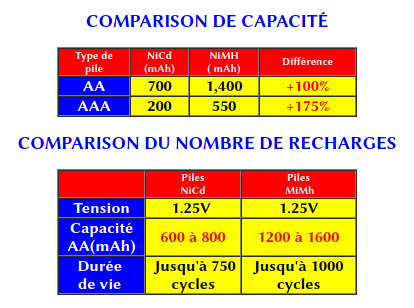
\includegraphics[width=11cm,height=\textheight]{images/comp.png}

\pagebreak

\hypertarget{quelles-autres-technologies-sont-couramment-employuxe9es-en-moduxe9lisme}{%
\subsubsection{2. Quelles autres technologies sont couramment employées
en
modélisme}\label{quelles-autres-technologies-sont-couramment-employuxe9es-en-moduxe9lisme}}

\begin{itemize}
\item
  Les batteries au plomb sont les moins chères des batteries (ancienne
  technologie peu performante et très polluante).
\item
  Les batteries Lithium ion ont une grande capacité de stockage dans un
  faible volume avec un faible poids. Elles possèdent une grande
  capacité massique. Ces batteries n'acceptent pas de surcharge sous
  peine d'exploser. Une gestion électronique est donc nécessaire.
\item
  Les batteries lithium polymère (Li-Po) sont une variante de la
  technologie lithium ion. Elles ont une densité énergétique et des
  caractéristiques à peu près similaires que les lithiums ion. Elles
  sont beaucoup utilisées dans le modélisme pour une question de poids.
  Cette technologie est un peu plus stable que le lithium ion. Sa
  recharge est plus compliquée et nécessite un chargeur adapté. Si la
  recharge n'est pas faite correctement la batterie prend feu. Son prix
  la rend moins attractive que la lithium ion.
\item
  Les batteries lithium fer phosphate (LiFePO4) stocke un peu moins
  d'énergie que la technologie lithium ion mais elle est entièrement
  stable, sans risque d'incendie ou d'explosion. Son point fort est son
  grand nombre de cycles. Elle est capable de réaliser 4 fois plus de
  charge/décharge qu'une batterie lithium ion classique et 5 fois plus
  qu'une batterie au plomb. Elle commence à être utilisée dans beaucoup
  de domaines industriels. Elle présente l'avantage d'avoir une tension
  proche d'une batterie 12V plomb (12,8V au lieu de 12V). Cette
  technologie devrait remplacer à terme les batteries plomb.
\end{itemize}

\pagebreak

\hypertarget{donner-la-fonction-de-ce-circuit-en-franuxe7ais.}{%
\subsubsection{3. Donner la fonction de ce circuit (en
français).}\label{donner-la-fonction-de-ce-circuit-en-franuxe7ais.}}

Ce circuit est un régulateur de tension.

Les régulateurs sont de très grande utilité dans les circuits
électriques lorsque vous avez besoin d'une tension stable. En effet un
régulateur permet de rentre la tension de sortie très fixe, ce qui est
préférable pour des composants comme les microcontrôleurs. Par exemple
pour un régulateur +5V, vous aurez au maximum une chute à +4.97V pour
des courants élevés. Ce qui est beaucoup plus précis que des piles ou un
adaptateurs secteurs 230V\textasciitilde{} -\textgreater{} 5V-.

Le régulateur de tension positive à 3 bornes LM7805 utilise un
limitation de courant interne, un arrêt thermique et une aire de
fonctionnement sécurisé. Avec un dissipateur thermique adapté, il peut
fournir un courant de sortie supérieur à 1A. Bien qu'il soit
initialement conçu comme un régulateur de tension fixe, ce dispositif
peut être utilisé avec des composants externes pour obtenir des courants
et des tensions ajustables.

\begin{itemize}
\tightlist
\item
  Courant de sortie jusqu'à 1 A
\item
  Protection contre les surcharges thermiques
\item
  Protection contre les courts-circuits
\item
  Aire de fonctionnement sécurisé des transistors de sortie
\item
  Aire de fonctionnement sécurisé des transistors de sortie
\end{itemize}

\hypertarget{donner-la-tension-de-sortie-du-lm7805.}{%
\subsubsection{4. Donner la tension de sortie du
LM7805.}\label{donner-la-tension-de-sortie-du-lm7805.}}

Tension de sortie: 5V

\hypertarget{donner-les-tensions-maximale-et-minimale-du-lm7805.}{%
\subsubsection{5. Donner les tensions maximale et minimale du
LM7805.}\label{donner-les-tensions-maximale-et-minimale-du-lm7805.}}

Tension minimale: 10V Tension maximale: 35V

\hypertarget{donner-les-courants-de-sortie-nominale-et-pic-du-lm7805.}{%
\subsubsection{6. Donner les courants de sortie nominale et pic du
LM7805.}\label{donner-les-courants-de-sortie-nominale-et-pic-du-lm7805.}}

Courant de sortie: 1A

\pagebreak

\hypertarget{quelles-cartes-du-vuxe9hicule-sont-alimentuxe9es-par-la-carte-alimentation}{%
\subsubsection{7.1 Quelles cartes du véhicule sont alimentées par la
carte alimentation
?}\label{quelles-cartes-du-vuxe9hicule-sont-alimentuxe9es-par-la-carte-alimentation}}

Les cartes alimentées sont les cartes, Maître, Esclave, Sirene et
Détection Piste

\hypertarget{quel-est-le-ruxf4le-de-la-capacituxe9-branchuxe9e-en-paralluxe8le-uxe0-lalimentation-sur-ces-cartes.}{%
\subsubsection{7.2 Quel est le rôle de la capacité branchée en parallèle
à l'alimentation sur ces
cartes.}\label{quel-est-le-ruxf4le-de-la-capacituxe9-branchuxe9e-en-paralluxe8le-uxe0-lalimentation-sur-ces-cartes.}}

La capacité branchée en parallèle fait office de filtre.

\hypertarget{comment-sont-alimentuxe9es-les-autres-cartes}{%
\subsubsection{8. Comment sont alimentées les autres cartes
?}\label{comment-sont-alimentuxe9es-les-autres-cartes}}

Les autres cartes sont alimentées par la batterie 1.

\end{document}
